\chapter{公式、图表、插图及代码}
\songti\xiaosi
\begin{spacing}{1.5}
	\section{图片使用}
	图片均放在figure目录下,在输入图片名称时,需要在前面添加“figure/”来确定路径。
	
	在某些情况下,如果不想让图片浮动把\fbox{[htb]}选项改成\fbox{[H]},H为强制禁止浮动,但会拉宽段间距和公式与正文之间距离。图片标题的格式和前后间距都已经设置,直接使用“$\setminus$caption”即可。
	
	\begin{lstlisting}
	\begin{figure}[htb]
	\centering
	\includegraphics[width=0.65\textwidth]{figure/fig_calculate}
	\caption{SampleFigure}\label{samplefigure}
	\end{figure}	
	\end{lstlisting}
	
	下图\ref{samplefigure}上面程序得到图片效果。
	
	\begin{figure}[htbp]
		\centering
		% Requires \usepackage{graphicx}
		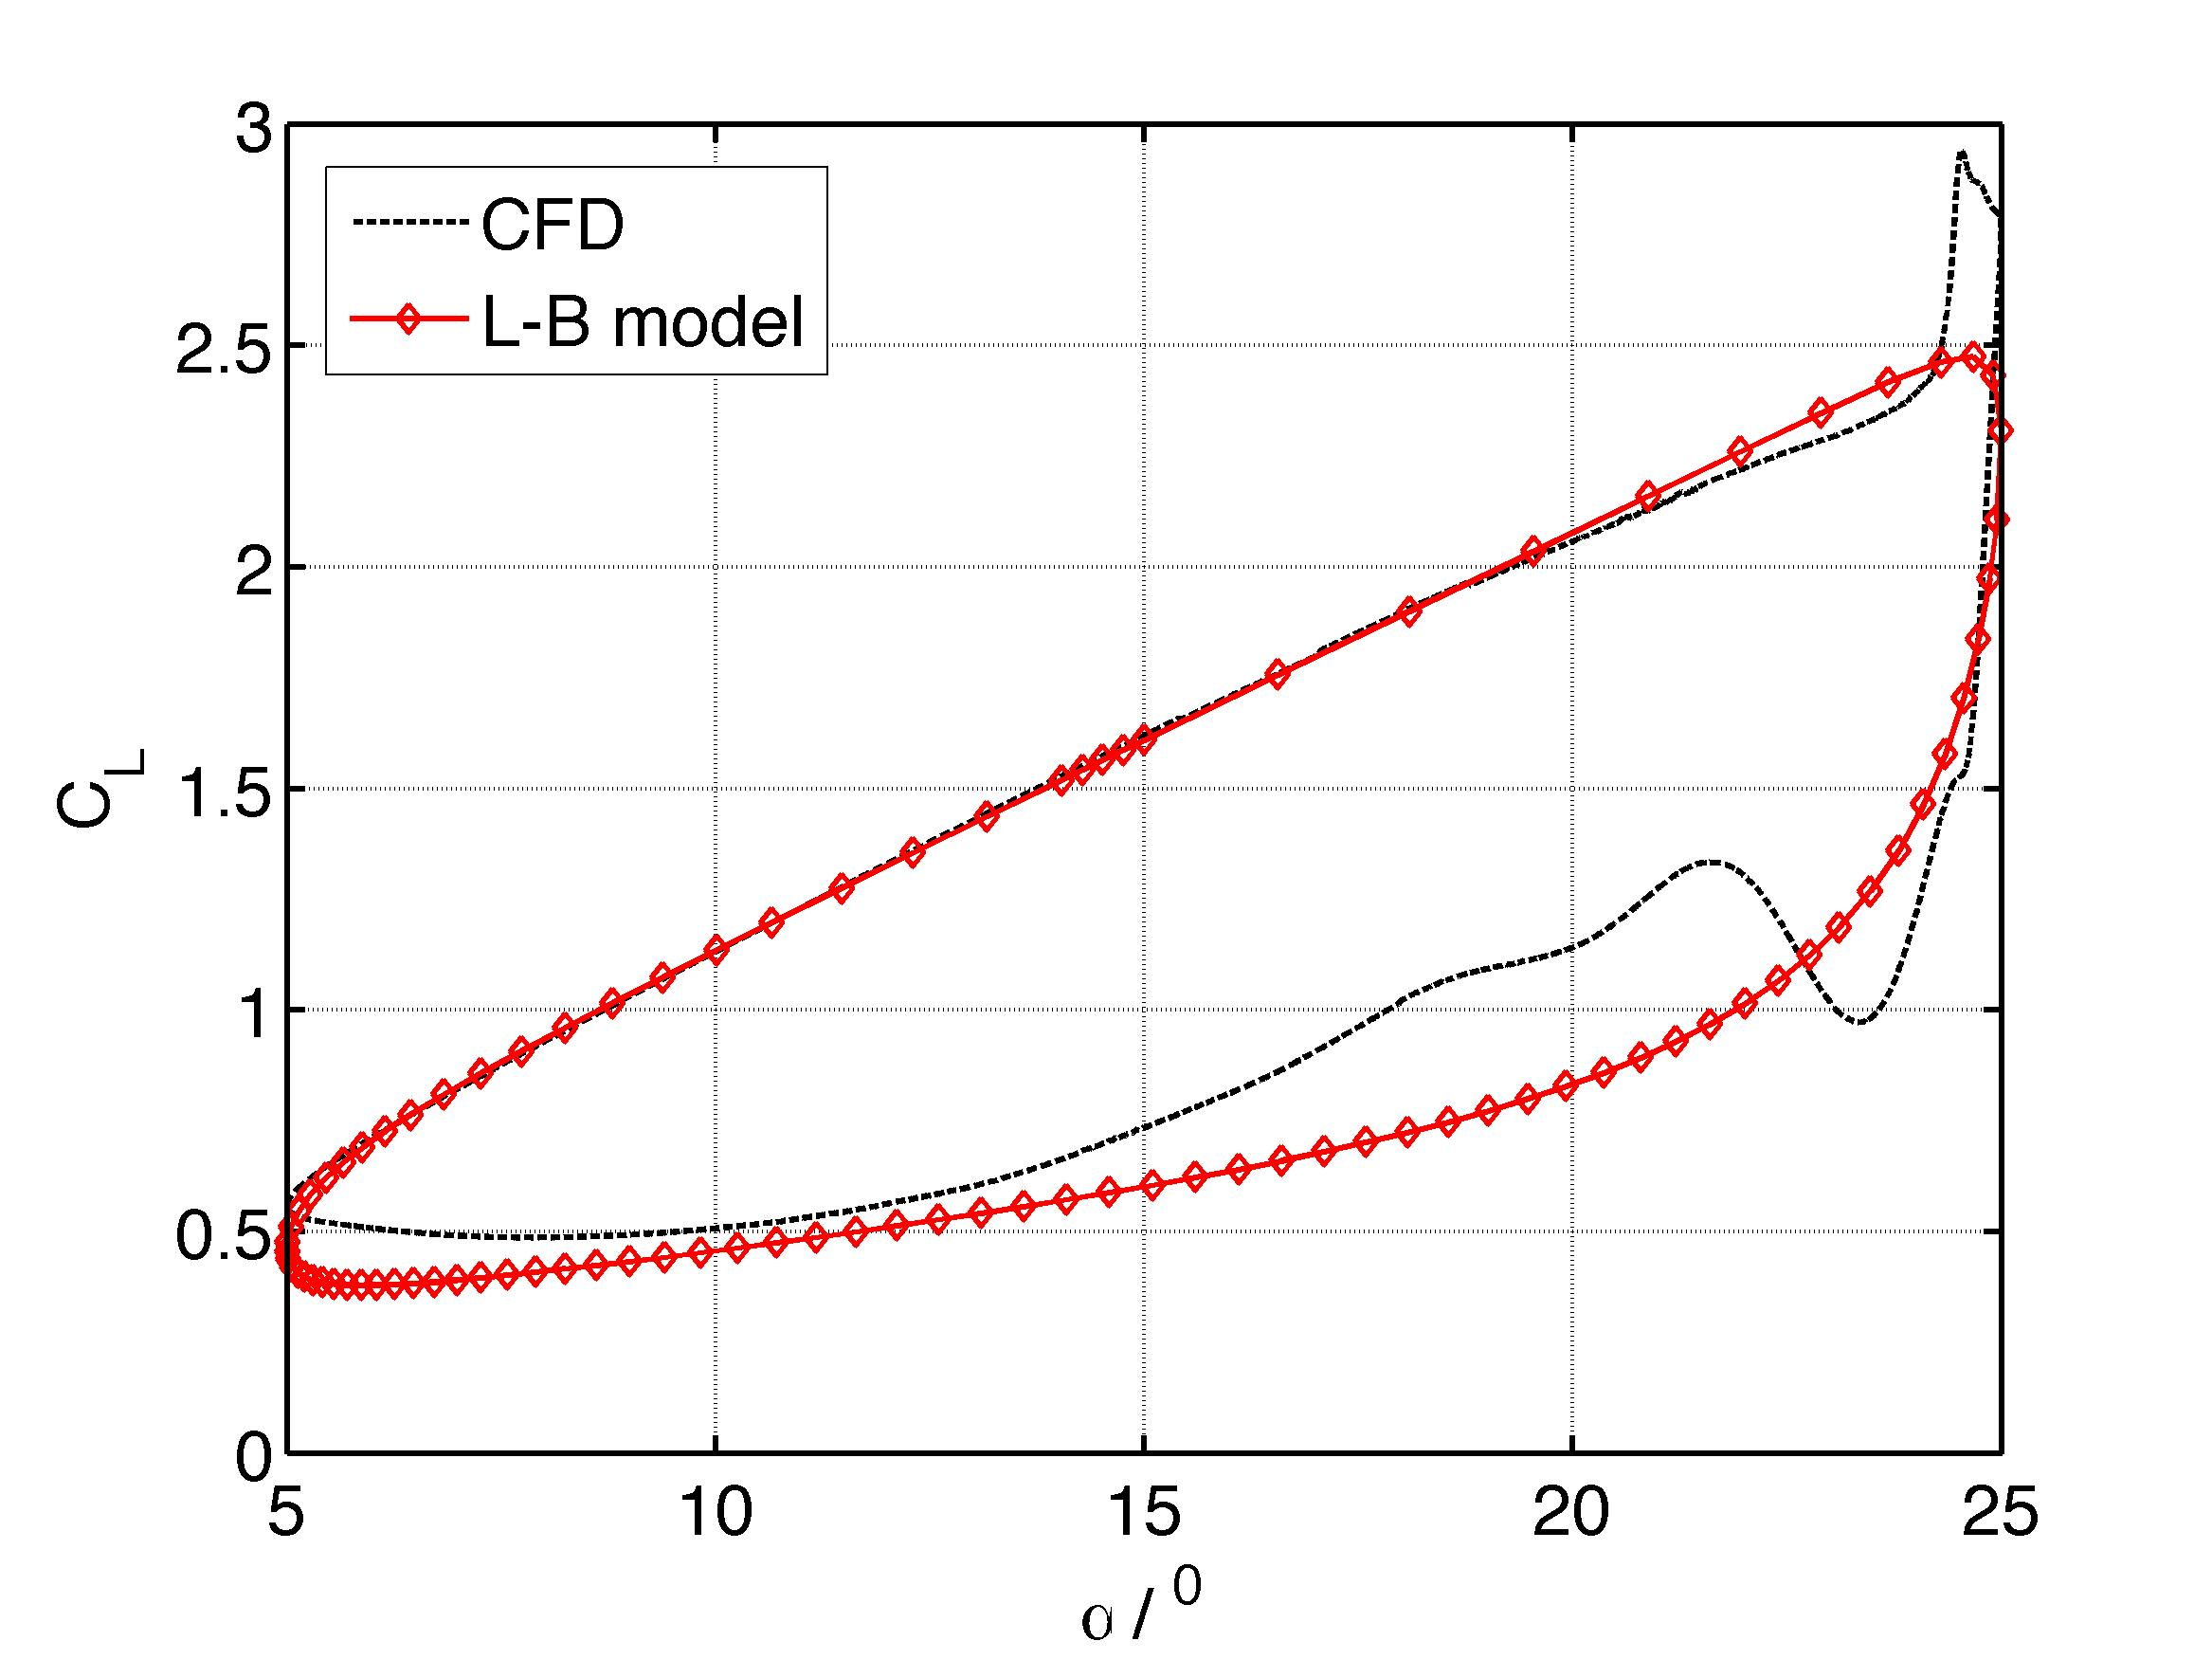
\includegraphics[width=0.65\textwidth]{figure/Curve_jpg}
		\caption{SampleFigure}\label{samplefigure}
	\end{figure}
	
	\section{表格使用}
	由于学校要求三线表格,自己在制作时需要注意该点,表格中的文字应该为五号宋体,结合两点要求,文本框中给出一个表格的范例。为了区分和图片的标题命名,在使用表格时使用“$\setminus$topcaption”,表格标题的格式和前后间距都已经设置。
	
	\begin{lstlisting}
	{\zihao{5}\songti
	\begin{table}[htb]
	\begin{center}
	\topcaption{SampleTable}\label{sampeltable}
	\begin{tabular}{m{3cm} m{2cm} m{2cm} m{2cm}}
	\hline
	Project & A & B & C\\
	\hline
	ProjectOne   & a1 & b1 & c1 \\
	ProjectTwo   & a2 & b2 & c2 \\
	ProjectThree & a3 & b3 & c3 \\
	ProjectFour  & a4 & b4 & c4 \\
	ProjectFive  & a5 & b5 & c5 \\
	\hline
	\end{tabular}
	\end{center}
	\end{table}}
	\end{lstlisting}
	
	下表\ref{sampeltable}是一个表格示例。
	
	{\wuhao\songti
		\begin{table}[htb]
			\begin{center}
				\topcaption{SampleTable}\label{sampeltable}
				\begin{tabular}{m{3cm} m{2cm} m{2cm} m{2cm}}
					\hline
					Project & A & B & C\\
					\hline
					ProjectOne& a1 & b1 & c1 \\
					ProjectTwo & a2 & b2 & c2 \\
					ProjectThree & a3 & b3 & c3 \\
					ProjectFour& a4 & b4 & c4 \\
					ProjectFive & a5& b5 & c5 \\
					\hline
				\end{tabular}
			\end{center}
	\end{table}}
	
	\section{公式使用}
	对于公式使用\fbox{$\setminus$begin\{equation\}}环境,如果有多行公式可以使用\fbox{$\setminus$begin\{split\}}环境,符号“\&”为各行公式对齐的位置。
	
	如果需要对公式中的字母进行注释,并且注释较多,这里推荐一种方法,可以使用表格的环境,表格为2列,第一列字母靠右,第二列解释靠左,如\fbox{$\setminus$begin\{tabular\}\{r@\{---\}l\}}。 
	下面文本框中给出了一个多行公式以及注释的示例。
	\begin{lstlisting}
	\begin{equation}\label{SampleEquation}
	\begin{split}
	\bm{x_}k&=\bm{\Phi}_{k,k-1}\bm{x}_{k-1}+\bm{\Gamma}_{k-1}\bm{w}_{k-1}\\
	\bm{z}_k&=\bm{H}_k\bm{x}_k+\bm{v}_k
	\end{split}
	\end{equation}
	\begin{tabular}{r@{---}l}
	$\bm{x}_k$  & The state variable of the $k^{th}$ step;\\
	$\bm{z}_k$  & The observation of the $k^{th}$ step; \\
	$\bm{\Phi}_{k,k-1}$ & The transition matrix of the $(k-1)^{th}$ to $k^{th}$ step; \\
	$\bm{\Gamma}_{k-1}$  & The measurement noise driving matrix of the $k^{th}$ step; \\
	$\bm{H}_k$  & The measurement matrix of the $k^{th}$ step;\\
	$\bm{w}_{k-1}$ & The systematic noise of the $(k-1)^{th}$ step ,$\bm{w}_{k-1}\sim N(0,\bm{Q}_{k-1})$;\\
	$\bm{v}_k$ & The measurement noise of the $k^{th}$ step,$\bm{v_k}\sim N(0,\bm{R}_k)$.
	\end{tabular}
	\end{lstlisting}
	下式\ref{sampeltable}和注释为上面程序的效果。
	\begin{equation}\label{SampleEquation}
	\begin{split}
	\bm{x_}k&=\bm{\Phi}_{k,k-1}\bm{x}_{k-1}+\bm{\Gamma}_{k-1}\bm{w}_{k-1}\\
	\bm{z}_k&=\bm{H}_k\bm{x}_k+\bm{v}_k
	\end{split}
	\end{equation}
	式中:
	\begin{tabular}{r@{---}l}
		$\bm{x}_k$  & The state variable of the $k^{th}$ step;\\
		$\bm{z}_k$  & The observation of the $k^{th}$ step; \\
		$\bm{\Phi}_{k,k-1}$ & The transition matrix of the $(k-1)^{th}$ to $k^{th}$ step; \\
		$\bm{\Gamma}_{k-1}$  & The measurement noise driving matrix of the $k^{th}$ step; \\
		$\bm{H}_k$  & The measurement matrix of the $k^{th}$ step;\\
		$\bm{w}_{k-1}$ & The systematic noise of the $(k-1)^{th}$ step ,$\bm{w}_{k-1}\sim N(0,\bm{Q}_{k-1})$;\\
		$\bm{v}_k$ & The measurement noise of the $k^{th}$ step,$\bm{v_k}\sim N(0,\bm{R}_k)$.
	\end{tabular}
	
	\section{代码插入}
	代码插入可以使用lstlisting宏包来实现,lsrlisting包中预置了一些常用语言的风格,可以直接在\fbox{$\setminus$begin\{lstlisting\}[language=]}中调用。我毕设中使用的是julia语言,并没有预置的环境而需要额外设置。在这里我直接使用了jlcode包中配置的环境,需要使用其他非预置语言环境的也可以寻找对应的环境包,或是自己手动进行配置(配置方法可以参照已有环境修改关键词和颜色)。
		
	lstlisting可以选择在latex中插入代码片段,或是直接从文件中读取,方式如下。
	
	\subsection{片段插入}
	\begin{lstlisting}
	\begin{lstlisting}
	function Style_3rd_Test(x, y)
	
	myver = v"2.00"
	mystr = "A string with \"Übergrößengeschäft\", α, π, ∪ and the + operator."
	myset = Set( [2, 9, 12, 25, 33])
	x_in_myset = x ∈ myset
	myset⁽²⁾ = myset ∪ Set( [4, 8, 12, 33])
	
	end
	 \ end{lstlisting}
	\end{lstlisting}
	效果如下:
	\begin{lstlisting}
	function Style_3rd_Test(x, y)
	
	myver = v"2.00"
	mystr = "A string with \"Übergrößengeschäft\", α, π, ∪ and the + operator."
	myset = Set( [2, 9, 12, 25, 33])
	x_in_myset = x ∈ myset
	myset⁽²⁾ = myset ∪ Set( [4, 8, 12, 33])
	
	end
	\end{lstlisting}
	
	\subsection{文件插入}
	
	\fbox{$\setminus$lstinputlisting\{code/testfile.jl\}}
	
	效果如下:
	\lstinputlisting{code/testfile.jl}
	\section{参考文献}
	参考文献在ThesisReference中\fbox{$\setminus$begin\{thebibliography\}}环境中进行填写,可以使用bibitem和BibTex两种方法。正文需要引用文献,使用\fbox{$\setminus$cite\{\}}即可。
	
	本文为了展示二者差别分别用两种方法进行了引用,实际应用中两种方式选一个即可。
	
	\subsection{bibitem}
	引言中前两个引用与第一页参考文献即为bibitem。格式如下:
	\begin{lstlisting}
	\begin{thebibliography}
	\bibitem author,article, year, vol,
	\end{thebibliography}
	\end{lstlisting}
	\subsection{BibTex}
	引言中后两个引用与第二页参考文献即为BibTex。
	
	进入谷歌学术、百度学术等文献检索网站,找到欲引用的文献页面并点击引用导出,选择BibTex导出。将导出内容保存成.bib文件并放到主程序相同目录中。
	
	在需要引用的位置使用fbox{$\setminus$cite\{\}}插入,并在需要显示参考文献的地方输入:
	
	\begin{lstlisting}
	\bibliographystyle{plain}
	
	\bibliography{ref}
	\end{lstlisting}
	
	使用TexStudio环境编译文件时,请在配置中将默认文献工具设为BibTex。若编译后未显示标号,可以尝试 latex-bib-latex 的三次编译法。
	
\end{spacing}